\documentclass{exam}
\usepackage{graphicx}
\usepackage{amsmath}

\begin{document}

\runningheadrule
\firstpageheader{Robot Control}{First Exam - Retake}{February 21, 2023}
\runningheader{Robot Control}{First Exam \thepage/\numpages}{February 6, 2023}
\firstpagefooter{}{}{}
\runningfooter{}{}{}

\begin{itemize}
    \item The theory part of the exam will be held from 11:00 to 11:45 and is worth 12 points.
    \item The practical part will be held from 12:00 to 14:00  and is worth 18 points.
    \item For the theoretical part of the exam, you are allowed to refer to your personal written notes. (no iPads)
    \item During the practical part of the exam, you are permitted to use your own equipment and consult online documentation. However, using sites such as Stack Overflow is not allowed.
    \item There are two tasks in theory part to be completed. Each task must be solved on a separate piece of paper and signed by you to confirm its completion.
\end{itemize}

\begin{questions}

\question

  Consider the following system, where $m, g, u_1, u_2$ are parameters of the system treated as constants (representing mass, gravity and fixed forces, 
  but the physical interpretation of the system is irrelevant from the problem's perspective).

  $$m\ddot{x} = -(u_1+u_2)\sin \theta$$
  $$m\ddot{y} = (u_1+u_2)\cos \theta -mg$$
  $$\ddot{\theta} = u_1-u_2$$


  \begin{parts}
    \part[1] Define system of equations that the fixed points have to satisfy.
    \part[2] The system can be solved only if the constants satisfy proper conditions. Solve the system and determine the conditions the constants have to satisfy so that at least one solution exist.
    \part[3] If you have properly determined the conditions, you will notice that there is an infinite number of solutions for the system. These can be divided into two classes of solutions depending on the theta coordinate of the fixed point. Linearise the system for each such class of solutions.
  \end{parts}

\begin{figure}[!ht]
\centering
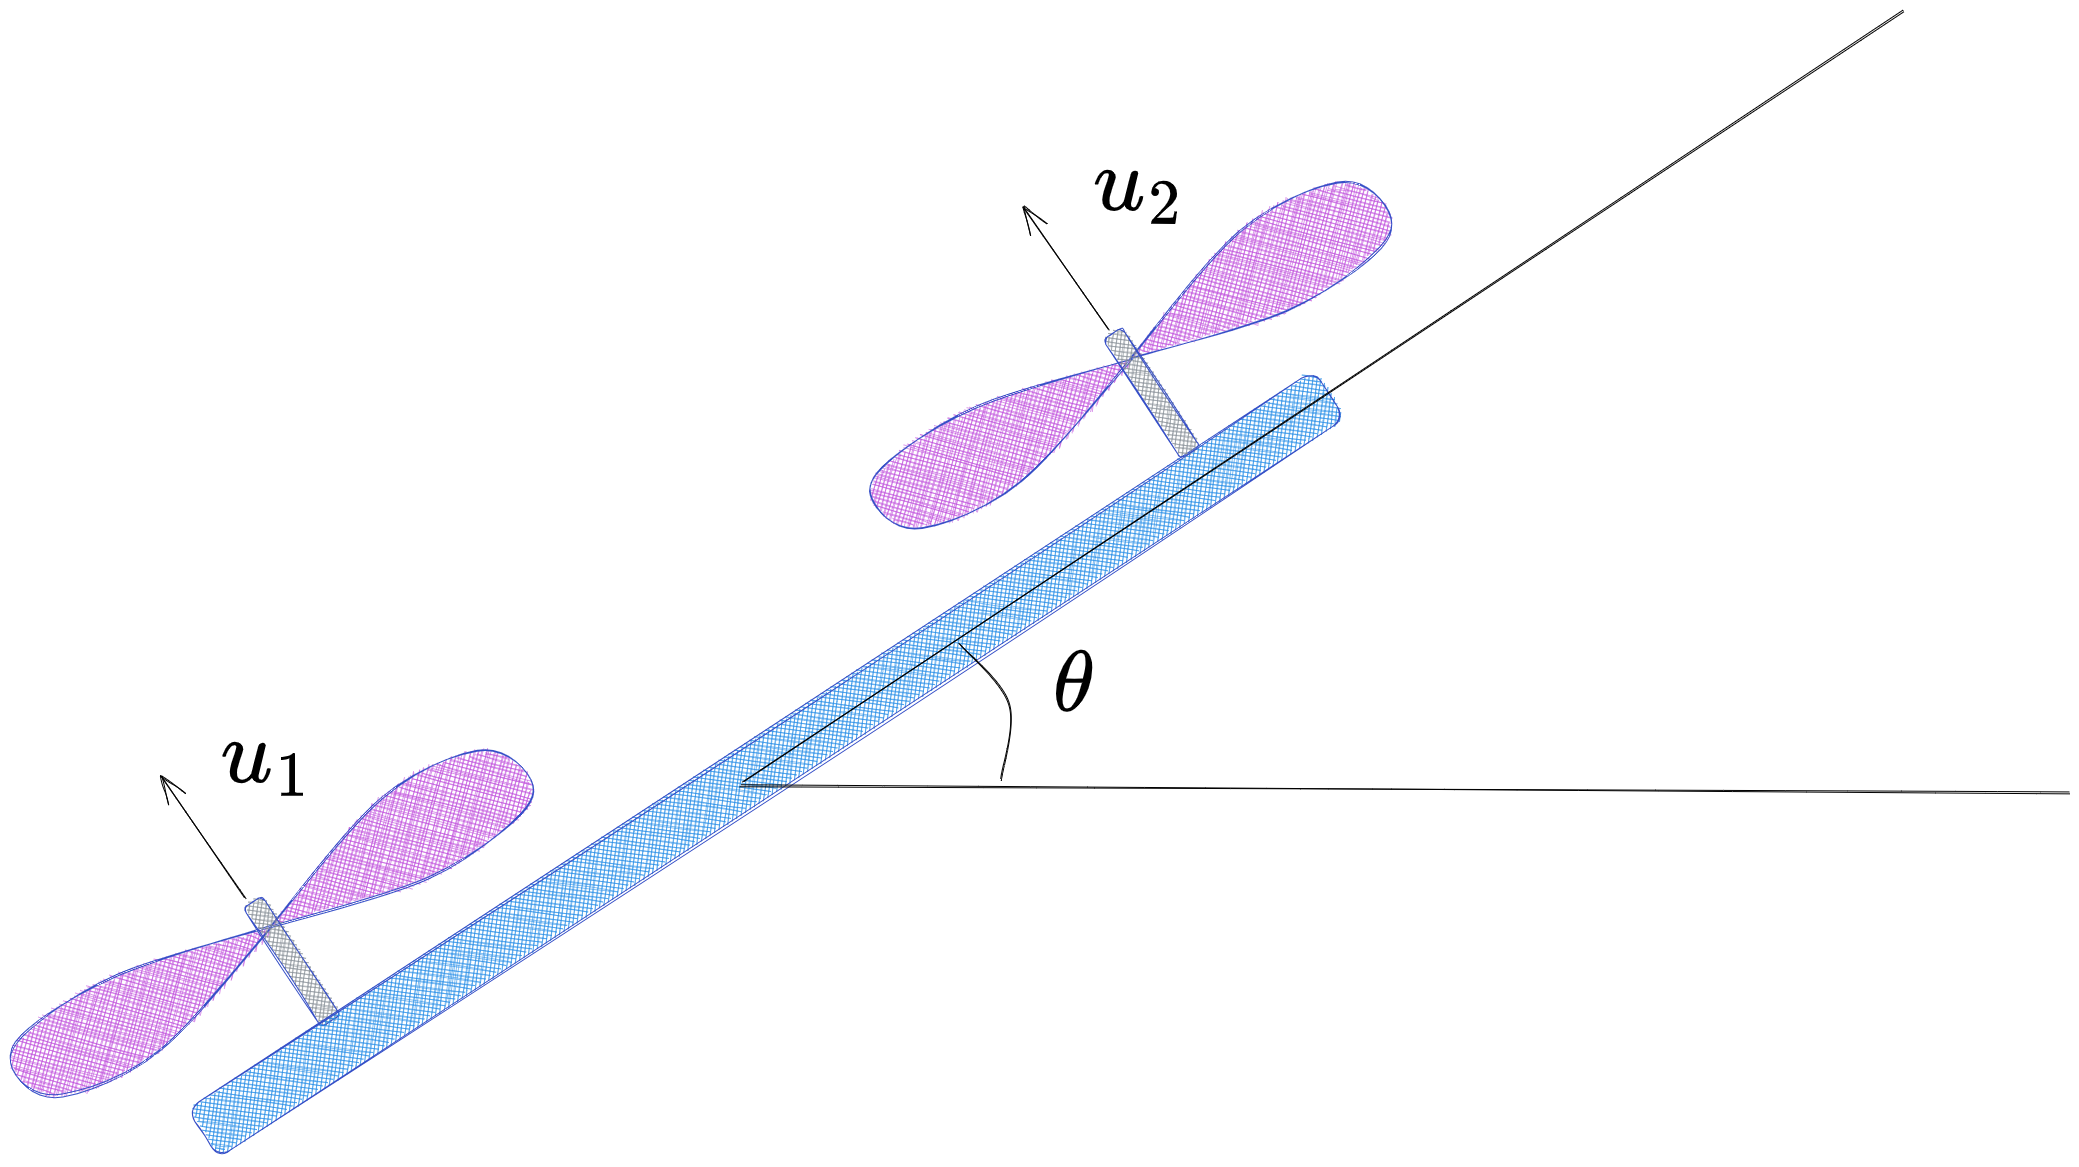
\includegraphics[scale=0.1]{drone.png}
  \caption{If you are looking for an interpretation of this system, it’s a simplified version of a system describing a drone which can move only on an XY plane where the Y axis is parallel to the direction of gravitational force, m is mass, g is the gravity of Earth and $u_1$ and $u_2$ are controls. Note that we assume additional constants (such as innertia) to be equal to 1, effectively ignoring the moments for the drone's rotation.}
\label{fig1}
\end{figure}

\question

\begin{figure}[!ht]
\centering
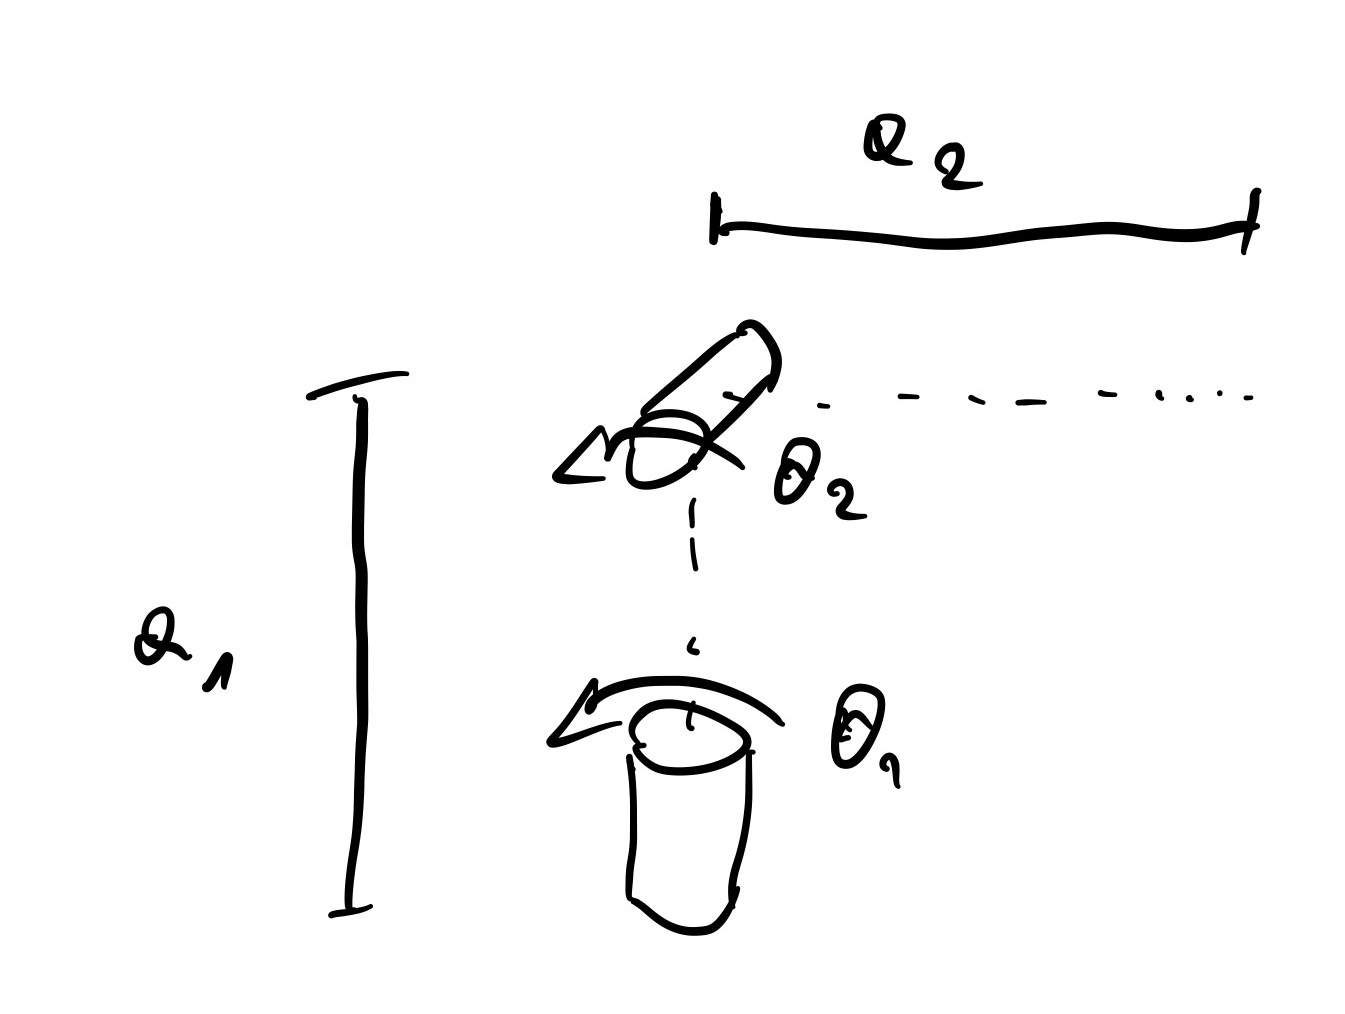
\includegraphics[scale=0.2]{task6.jpg}
\caption{Kinematic chain for problem 2.
  Note that the axis along the second link is perpendicular (and not parallel), to the axis of rotation of the second joint.}
\label{fig2}
\end{figure}

Given the visual description of the kinematic chain (figure \ref{fig2}), with two degrees of freedom $\theta_1$ and $\theta_2$
do the following:

\begin{parts}
\part[1]
  Find the forward kinematics $FK(\theta_1, \theta_2)$ of the robot.
\part[1]
  Find the workspace of the robot for given $a_1, a_2$.
\part[1]
  Find the inverse kinematics $IK$ of the robot.
\part[1]
  Assign frames to the joints of the kinematic chain using the  DH-convention.
\part[2]
  Create the DH-table for the kinematic chain.
\end{parts}

\end{questions}

\end{document}

